%!TEX root = ../report.tex

This chapter explores the design of the system by first introducing the main system components that comprise the application. Following this, the requirements for the user interface are refined before the user actions and activities are investigated. Next, the development methodology, design patterns, non-functional requirements and the dataset design are discussed. At the end of this chapter, the design of system evaluations is examined.

\section{System components} {
\label{sec:system_components}

	The application consists of five high-level modular components, which can be seen in Figure~\ref{sec:system_components} and are described below. This design decision ensures that a module can be removed from the application at any time, without effecting the other modules.

	\begin{description}[leftmargin=0pt]
		\item[Navigation:] The navigation interactions between the user and the visualisation including pan, zoom and rotate.
		\item[Visualisation:] The visualisation encompasses the 3D environment viewed by the user.
		\item[Information:] The information component refers to additional information pertaining to the dataset that can be viewed by the user. This component is supported by utilising metadata in the dataset.
		\item[Filtering:] This component is responsible for filtering data in the visualisation. It controls the visibility of data points and their information.
		\item[Configurations:] Settings that modify the appearance of the visualisation.
	\end{description}

	%!TEX root = ../../report.tex

\begin{figure}[H]
	\centering
    \includegraphics[width=\textwidth]{images/design/system_components}
    \caption{System component diagram.}
    \label{fig:system_components}
\end{figure}


}

\section{User interface} {
\label{sec:user_interface}

	The graphical user interface (GUI) for this system has combined Google's Material Design~\footnote{\bibentry{google2015material}} with a 3D environment, to simplify the way users interact with the system.

	\subsection{Material Design} {
	\label{sec:material_design}

		Material Design is a visual language developed by Google that synthesises classic design principles with current technologies. Their design aims to provide users with a unified experience across platforms and device sizes, by focusing on user actions and retaining continuity between transitions. Furthermore, Material Design provides an immersive experience to users by adhering to good design principles.

		Google Material Design details many component specifications that have been implemented by several CSS3 frameworks. It is also a great design tool that has been incorporated into both the existing infrastructure of this project and the group project.

		% As a result of this, a user can transition from one system to the other seamlessly, because both systems apply the same design standards.

	}

	\subsection{3D environment} {
	\label{sec:3d_environment}

		The visualisation viewed by a user features a 3D environment which has been designed with the following in mind:

		\begin{itemize}
			\item Data point displays that represent the dataset are displayed as 3D bars.
				\begin{itemize}
					\item These displays should have the ability to be filtered.
				\end{itemize}
			\item The colour of a data display can be configured and should be effected by the value it represents.
				\begin{itemize}
					\item e.g. Data displays that represent population data may be coloured red, orange or yellow to indicate high, medium or low population areas respectively.
					\item Colour accessibility issues are reduced by enabling the user to modify the colours of the data display.
				\end{itemize}
			\item Information associated with a data display can be viewed by a user, either through hover effects or by outputting the dataset on the page.
				\begin{itemize}
					\item The interface should use a simple panel interface, shown in Figure~\ref{fig:information_display_design}.
				\end{itemize}
			\item Data displays appear projected from a base geometry, either a cuboid or sphere depending on the dataset being used.
			\item A skybox should serve as a static background for the environment.
		\end{itemize}

		%!TEX root = ../../report.tex

\begin{figure}[H]
	\centering
	\newcommand{\figurewidth}{0.4\textwidth}
	\centering
	\begin{subfigure}[b]{\figurewidth}
        \figureborder{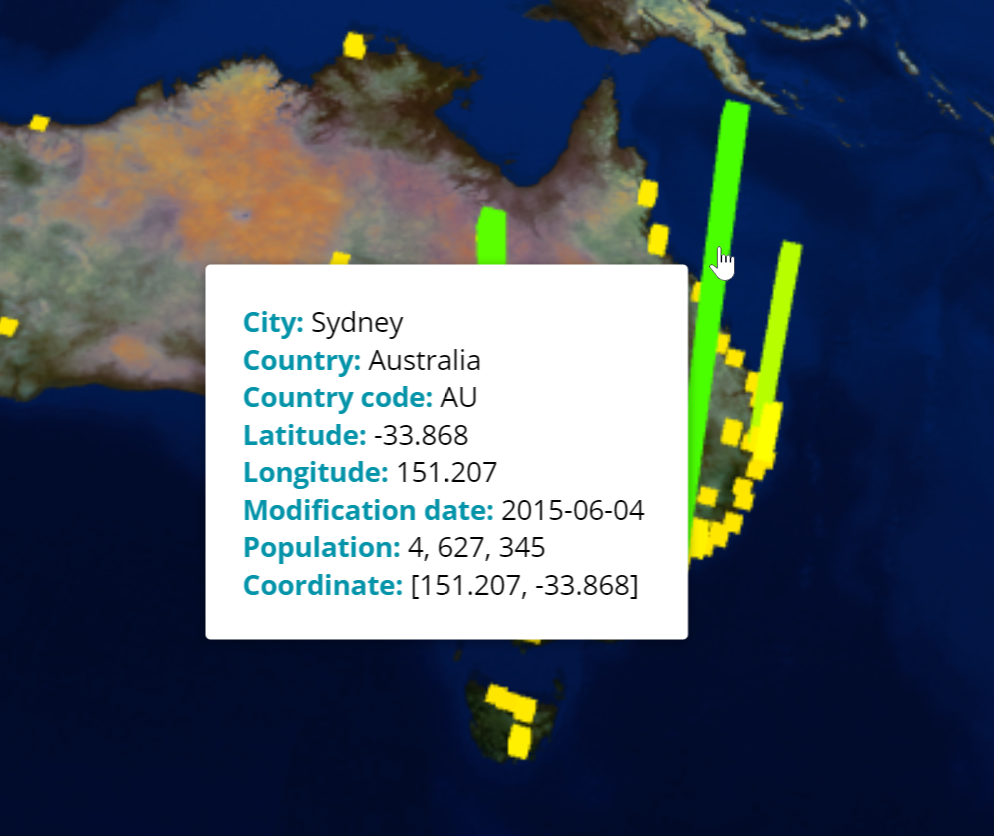
\includegraphics[width=\textwidth]{images/implementation/information_display/population}}
		\caption{Information display for population data.}
		\label{fig:information_display_population}
	\end{subfigure}
	\begin{subfigure}[b]{\figurewidth}
		\figureborder{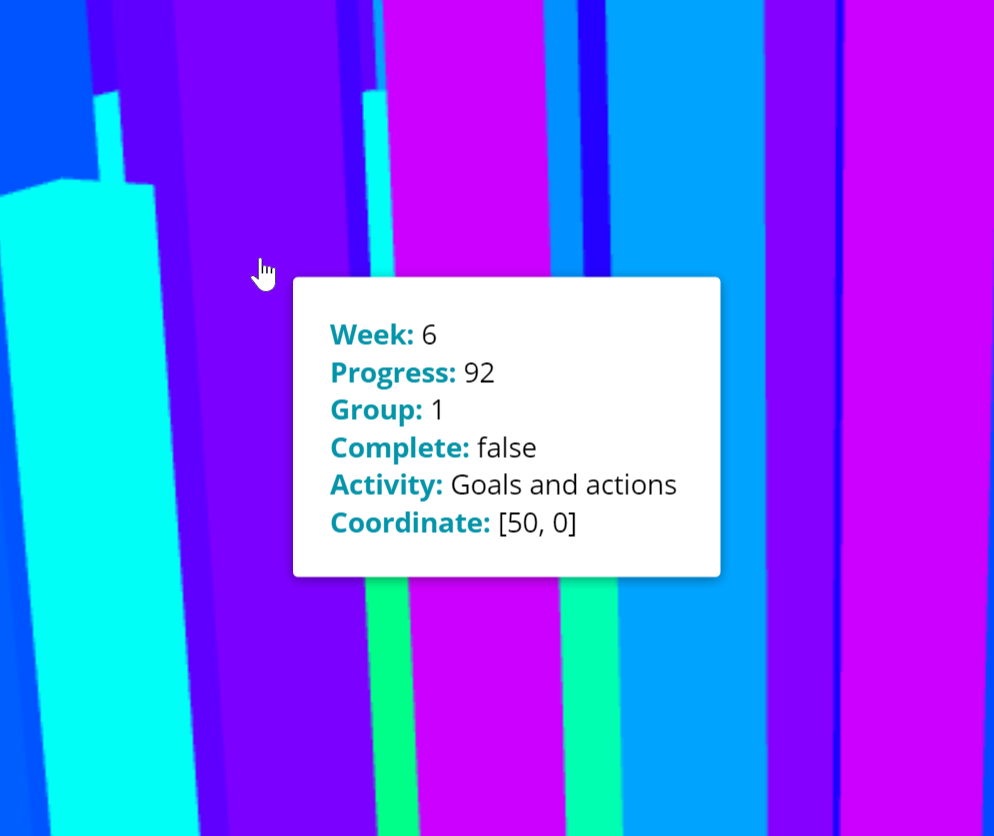
\includegraphics[width=\textwidth]{images/implementation/information_display/student}}
		\caption{Information display for student data.}
		\label{fig:information_display_student}
	\end{subfigure}
	\caption[Information display]{Information display hover effect.}
	\label{fig:information_display}
\end{figure}


		Example mockups of the 3D environment that fulfil the above criteria have been demonstrated in Figure~\ref{fig:environment_mockups}.

		%!TEX root = ../../../report.tex

\begin{figure}[H]
    \newcommand{\figurewidth}{0.5\textwidth}
    \newcommand{\figureheight}{3cm}
	\begin{subfigure}[b]{\figurewidth}
        \centering
        \raisebox{0.5\height}{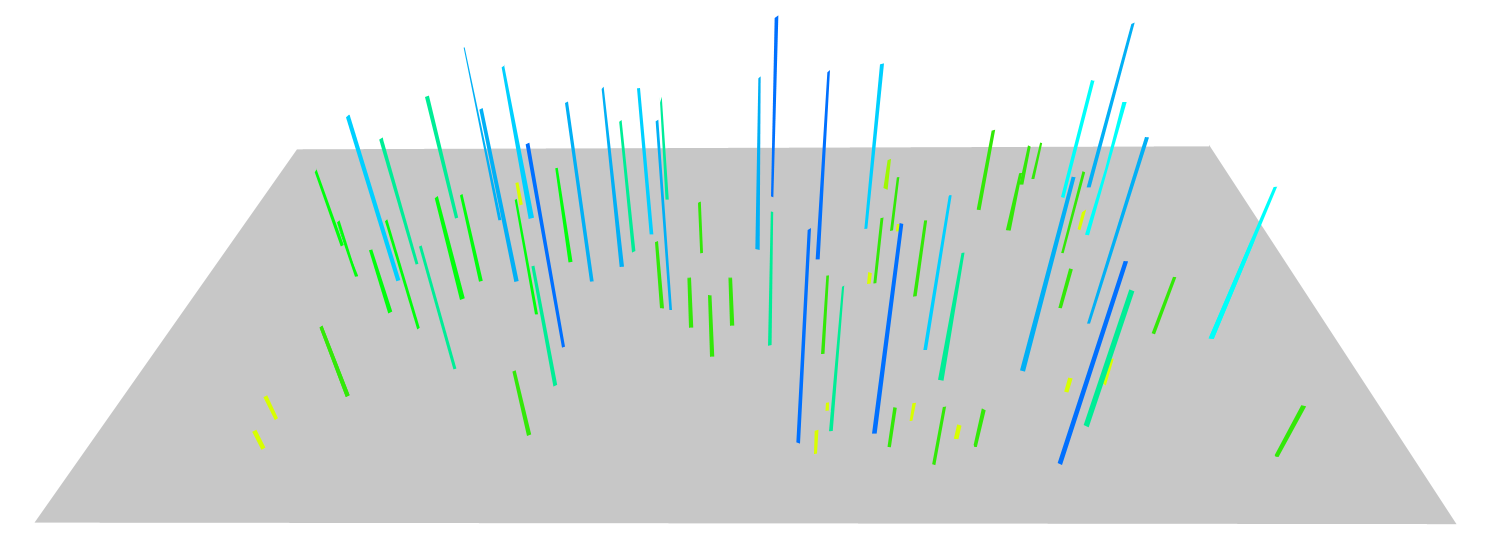
\includegraphics[width=\textwidth]{images/design/mockups/flat}}
        \caption{Visualisation using a flat surface.}
        \label{fig:visualisation_flat}
    \end{subfigure}
    \begin{subfigure}[b]{\figurewidth}
        \centering
        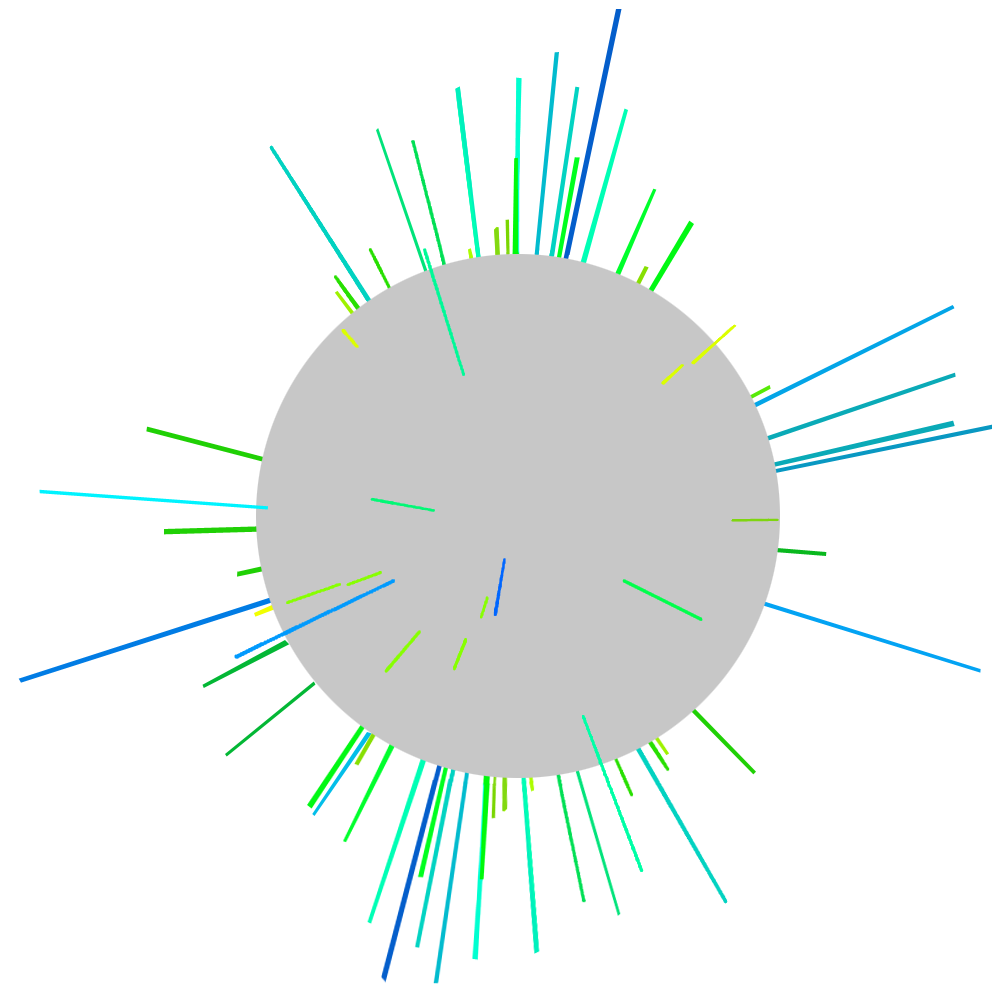
\includegraphics[width=\textwidth]{images/design/mockups/sphere}
        \caption{Visualisation using a sphere surface.}
        \label{fig:visualisation_sphere}
    \end{subfigure}
	\caption[3D environment mockups]{3D environment mockups.}
	\label{fig:environment_mockups}
\end{figure}


	}

	\subsection{Interface design} {
	\label{sec:interface_design}

		The design of the interface needs to account for both the use of Material Design and the 3D environment. 

		Material Design is renowned for its sliding drawer menu, often used to maximise the viewing space for the user. This component has the potential to maintain user focus on the visualisation, while providing additional information through an unobtrusive menu. An initial mockup of this design has been demonstrated in Figure~\ref{fig:user_interface_mockup}, where the 3D environment fills the content to the right of the drawer. This design has been refined through the implementation phase described in Section~\ref{sec:filtering_implementation} and \ref{sec:configuration_implementation}.

		%!TEX root = ../../../report.tex

\begin{figure}[H]
	\centering
    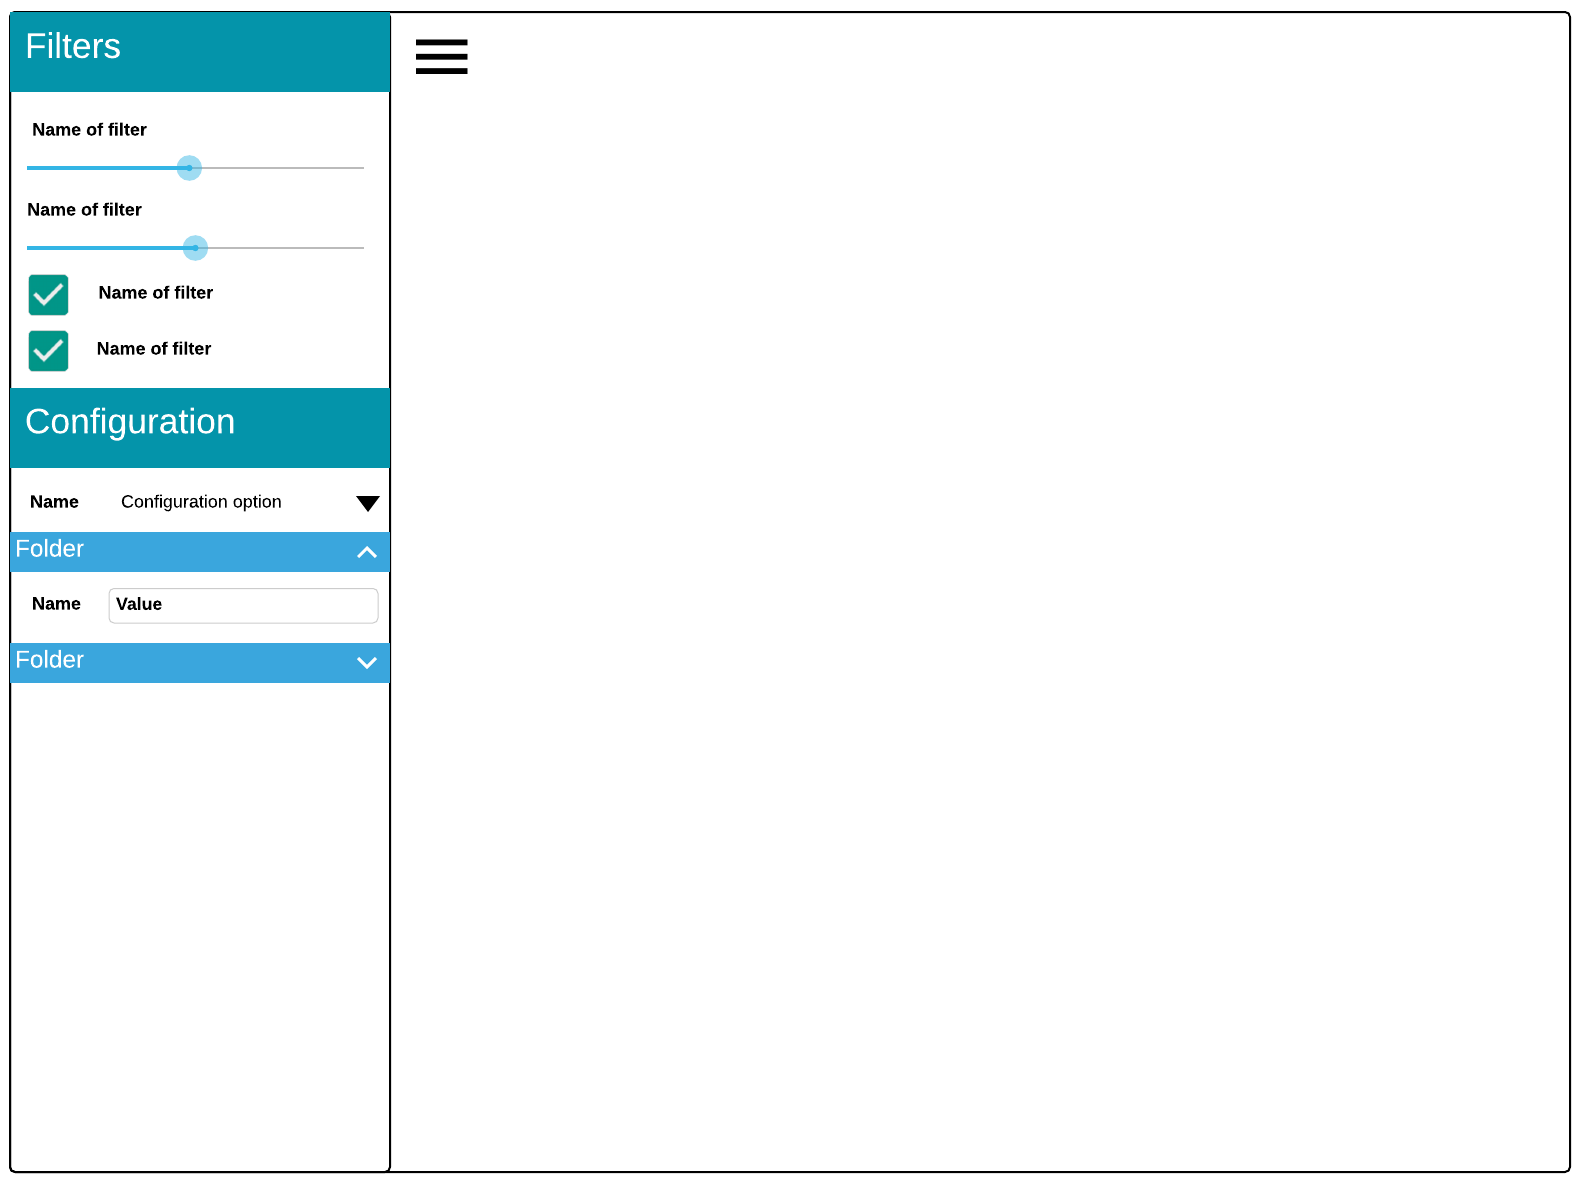
\includegraphics[width=\textwidth]{images/design/mockups/interface}
    \caption[User interface mockup]{User interface mockup.}
    \label{fig:user_interface_mockup}
\end{figure}


		The sliding drawer utilises Material Design components and incorporates two main features -- filtering and live configuration.

		\subsubsection{Filtering} {
		\label{sec:filtering}

			Filters take advantage of slider and checkbox widgets to adjust the state of what is displayed to the user. Their purpose is to provide users with the ability to identify characteristics of the dataset more quickly. For example, the data displays for a population dataset could be filtered so that cities of particular population, longitude or latitude range are visible. The user could then perhaps identify which cities are densly populated in certain regions on the world map. 

			\emph{Sliders} adjust what data displays are visible to the user. This is achieved by configuring the bounds of the available metadata in the data model. Take for example a dataset that has a range of values between 0 -- 100. If the user adjusts the value of its respective slider to be $\ge$20, then any data displays that have a value \textless20 will be hidden. As the ranges of a dataset become very small and precise (e.g. 0.001 -- 0.01) or large (e.g. 1,~000,~000 -- 1,~000,~000,~000), the step size for a slider may need to be adjusted to account for such values. In the case of small and precise ranges the step size may default to integer increments. This would become problematic for the user as the slider cannot be adjusted to decimal values. Similarly, for large ranges the user may wish to utilise larger increments as smaller step sizes could introduce performance issues when filtering on each unique value.
			
			\emph{Checkboxes} are designed to be toggled on or off. This widget toggles what metadata associated with a data display is shown to the user.

		}

		\subsubsection{Configurations} {
		\label{sec:configurations}

			Configuration options are designed to change the values and attributes of the 3D environment in real-time, promoting the analysis of the effects colour has on usability and identifying pertinent information. These options are organised in a folder structure, to deliver a hierarchy and logical grouping to the user. Moreover, these options should handle configuring data displays and surface values which enable the user to customise the display of the system.

			\emph{Data display} configurations should modify the low, medium, high colour values and the range of colours displayed.

			\emph{Surface} configurations should modify the midtone colours of the surface and the colour or intensity of other surface attributes.

		}

	}

}

\section{User actions} {
\label{sec:user_actions}

	The interactions that a user can perform when using this system have been represented in Figure~\ref{fig:user_actions}.

	%!TEX root = ../../report.tex

\begin{figure}[H]
	\centering
    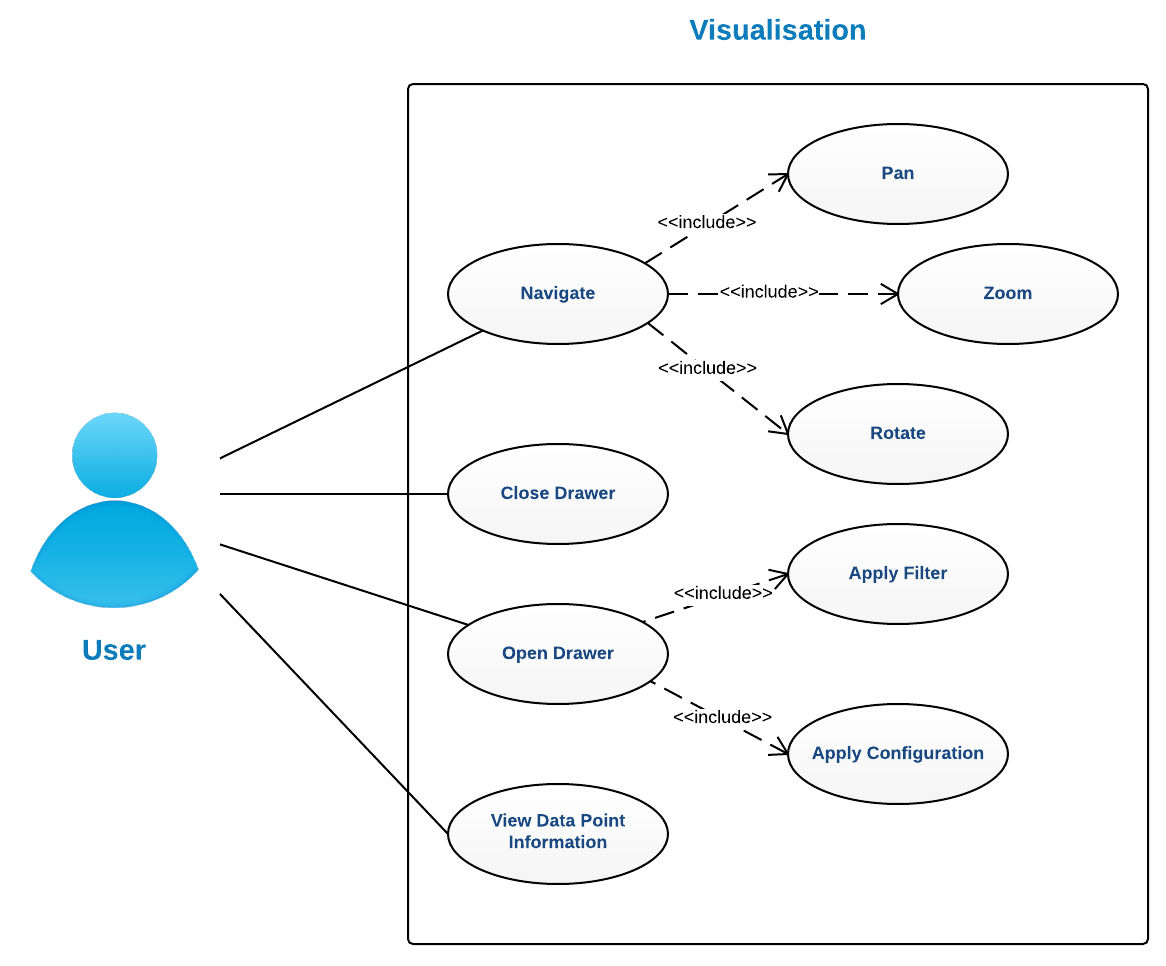
\includegraphics[height=10cm]{images/design/user_actions}
    \caption[User actions]{User actions use-case diagram.}
    \label{fig:user_actions}
\end{figure}


	These user actions facilitate decision making processes by allowing users to evaluate the dataset loaded with a visualisation in order to identify key features. For instance, when the user navigates around the scene they are able to view the information associated with a data display by hovering on it. In regards to population data the smallest and largest city or country can be established using this method. This is achieved by navigating to a short or tall data point and displaying its information which contains details such as the city and country. Similarly, when a student dataset is used the best and worst performing groups can be identified on a weekly and on an average basis by analysing this information. Viewing student progress in such a manner can also aid in determining patterns with particular groups and individuals, and examining the overall complexity of a task during certain weeks. 

	When filtering is applied to any dataset, the user can confirm their initial observations found during the navigate and view data point information actions. This is due to the fact that a filter can determine which data displays are visible to the user, by adjusting the minimum and maximum range of a property in the dataset through a widget. As an example, displaying populations that are either below or over 100,~000 individuals can easily be seen by adjusting the minimum or maximum filter bounds for the population property to 100,~000.

	Finally, different configurations can be applied to customise the appearance of the environment. This is done so that a distinguished colour scheme for the data displays and surface is selected. In turn, this can enhance a user's ability to identify significant features and patterns through colour palettes that make the dataset clearer to understand.

}

\section{Methodology} {
\label{sec:methodology}

	A rapid application development (RAD) approach~\parencite{martin1991rapid} was undertaken when developing this project as it promotes iterative development and the rapid construction of prototypes. This software methodology is flexible and can respond to changing requirements because less time is invested into planning the project. This contrasts with the traditional waterfall~\parencite{huo2004software} approach which places greater emphasis on planning, gathering requirements, scheduling and following a rigid workflow. RAD instead enables the software to be written quickly through the reuse of software components and engaging in less formal reviews. The RAD model has been shown in Figure~\ref{fig:rad}.

	%!TEX root = ../../report.tex

\begin{figure}[H]
	\centering
    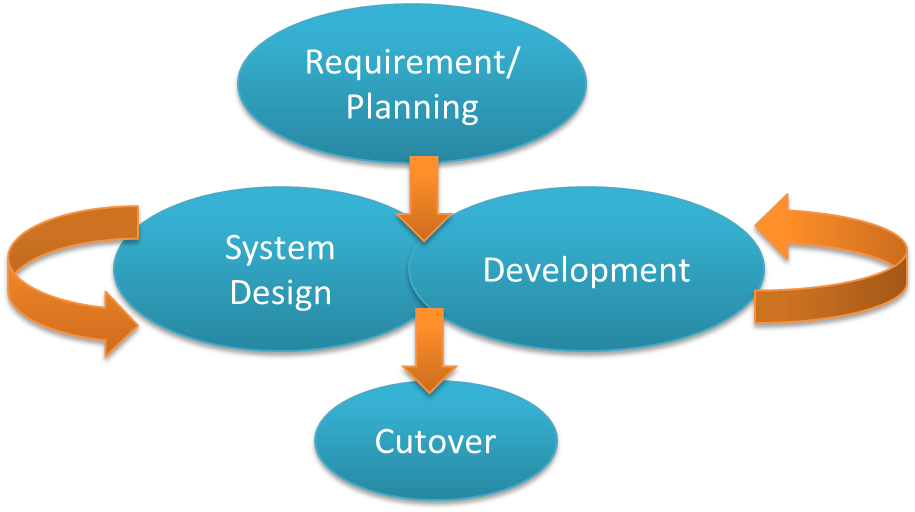
\includegraphics[height=6cm]{images/design/rad}
    \caption[Rapid application developement]{Rapid application developement model~\protect\footnotemark.}
    \label{fig:rad}
\end{figure}

\footnotetext{\bibentry{javatechig2012rad}}


	In this project, each visualisation can be thought of as a single prototype, where parts of a prototype can be reused for the next visualisation. Testing should be performed during the course of the project, but particularly when a major component of a prototype has been developed, such as data filtering.
		
}

\section{Design patterns} {
\label{sec:design_patterns}

	This system has combined asynchronous event-driven programming, through the Observer pattern~\parencite{osmani2012learning}, with the Model-View-Controller~\parencite{krasner1988description} (MVC) design pattern to create a modular application.

	Event-driven programming is a programming paradigm where the flow of the program is determined by events which include user actions or messages from other programs. This paradigm is suited to web applications as actions can be performed in response to user input such as mouse clicks and keyboard input. Moreover, event-driven programming promotes the implementation of loosely-coupled modules.

	The role of the MVC design pattern is to separate the concerns between the representation of information from the way this information is presented and manipulated by the user, as shown in Figure~\ref{fig:mvc}. This pattern also increases the scalability, maintainability and extensibility of applications.

	%!TEX root = ../../report.tex

\begin{figure}[H]
	\centering
    \includegraphics[width=0.7\textwidth]{images/design/mvc}
    \caption{Model-View-Controller design pattern.}
    \label{fig:mvc}
\end{figure}


}

\section{Non-functional requirements} {
\label{sec:non_functiona_requirements}

	The following non-functional requirements are considered key to the success of this project:

	\begin{description}[leftmargin=0pt]
		\item[Modularity:] The project should be highly modular, so parts of the system can be reused and easily integrated into the group project.
		\item[Performance:] The response time of the system is a major concern when working with a large dataset. The time to load the visualisation is highly dependent on the size of the dataset, graphical processing, network bandwidth and latency. However, once the visualisation has loaded, the user should be faced with near immediate response times (\textless 1 second).
		\item[Scalability:] This is important when modifying the size of the dataset used with a visualisation. The visualisation should be capable of handling increased processing with a larger dataset. Not only this, but the information should remain mapped to the correct locations in the scene with increased volumes of data.
		\item[Testability:] Highly testable code is important when writing test suites, so all aspects of the system can be easily tested to locate faults. In JavaScript:
			\begin{itemize}
				\item A common technique is to hide variables through the use of closure, which leads to untestable code. These variables should be replaced with public variables that are prefixed with an underscore, to indicate they are not a part of the public API.
				\item Promises should not be used within a constructor.
				\item Anonymous functions should be replaced with named functions so they can be tested.
				\item Dependency injection should be handled through a module loader.
			\end{itemize}
	\end{description}

}

\section{Dataset} {
\label{sec:dataset}

	As discussed in Section~\ref{sec:project_definition}, the visualisations began with generated data so development could begin immediately. Using generated data brings control over the size of the dataset applied to a prototype and the scalability of each visualisation can be tested. Following the use of fake data, each prototype had real datasets applied to them. GeoNames~\footnote{\bibentry{wick2005geonames}} is a geographical database that was used for the implementation of the visualisations. This database stores population data for a significant number of cities and their respective latitude and longitude coordinates. GeoNames falls under a creative commons attribution license, so there are no copyright concerns or immediate issues when reading and parsing the data it provides. However, some information contained in this dataset (such as \emph{geonameid}, \emph{feature class} and \emph{dem}) are not necessary to be included for processing and when viewed by the user. Furthermore, the format of this dataset is not appropriate for parsing. The tab separated list should be converted to a JSON structure so the data can be read efficiently in order to reduce the loading time for the user. Once real datasets had been applied to the visualisations, the system was integrated with a student progress dataset to provide an analytics component for teachers.

	Initially, a flat array structure was considered for the design of the dataset as it is significantly more performant to parse than objects, as shown in Figure~\ref{fig:performance_test}. However, this structure is inflexible and difficult to maintain as a result of its rigid format. The use of objects are a more flexible, albeit less performant, structure that was considered in the design of the dataset. When using objects, a key can be selected as a value to be used for the x, y and z axis. Another advantage to using objects is that metadata can easily be added to the dataset. While there are certainly tradeoffs between the two structures, the flexibility of objects was valued over performance differences that would only occur during application startup. Due to these reasons, objects were used to form the structure of the datasets.

	%!TEX root = ../../report.tex

\begin{figure}[H]
	\centering
    \figureborder{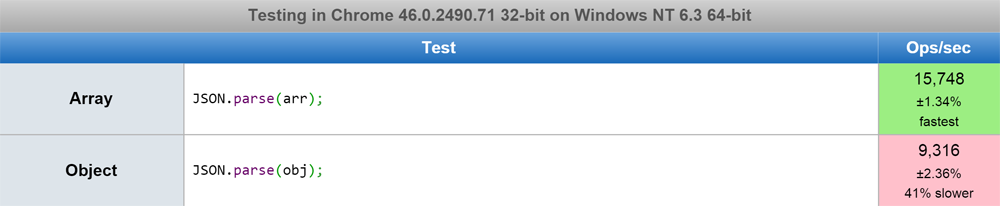
\includegraphics[width=0.7\textwidth]{images/design/performance_test}}
    \caption[Performance test]{Performance test between array and object data.}
    \label{fig:performance_test}
\end{figure}


}

\section{Evaluation design} {
\label{sec:evaluation_design}

	It is important to measure the usability of the system and the tools it offers, so users can effectively interpret the information presented to them in an attempt to aid data exploration and decision-making processes. Performance plays a significant role toward the usability of the system, as it ultimately determines how responsive the system appears to the user. Both the usability and performance of the system can be assessed by performing a user study and performance evaluation respectively.

	The user study has been designed to include a questionnaire and System Usability Scale, which both aim to assess the usability of the system. The objective of the questionnaire is to collect information from the user regarding their experience when using the system. The user is also asked to perform two activities and answer whether they used filtering to discover this information. Similarly, the System Usability Scale~\parencite{brooke1996sus} is a tool for measuring the usability of a system. This scale consists of a simple ten item questionnaire and is designed to be answered by respondents quickly and easily. Furthermore, the System Usability scale has become an industry standard by yielding reliable results and can be viewed in Appendix~\ref{app:system_usability_scale}.

	This study has been limited to the students enrolled in the final year project. It is required that the participants sign a consent form before they evaluate the system. Likewise, the participants must be informed of how the confidentiality of the research data will be maintained. This will be supported by anonymising the research data such that the participants cannot be identified from the results presented in this thesis.

	The performance and scalability of the system has been designed to be tested in an offline environment on a single high performance computer. The metrics for evaluating the performance and scalability of the system include the time to load, time to perform filtering and the average frames per second when idle and navigating the scene. These metrics have been recorded for each visualisation across small ($\approx$ $\le5000$) and large ($\approx$ $\ge10000$) datasets.

}

This thesis has illustrated the design of the system which takes a rapid application development approach to implement the visualisations using event-driven programming and the MVC design pattern. The system consists of five highly modular components including the navigation interactions, the 3D environment and dataset information, data filtering and configuration settings. Modern interface design principles have been incorporated into the design which have been presented through design mockups. Moreover, there are also several activities that the user can undertake based on the dataset used with the visualisation.
